\documentclass[11pt]{article}

\usepackage[review]{acl}

\usepackage{times}
\usepackage{latexsym}
\usepackage[T1]{fontenc}
\usepackage[utf8]{inputenc}
\usepackage{microtype}
\usepackage{inconsolata}
\setlength{\emergencystretch}{3em}
\hyphenation{sal-u-ta-tion in-con-sis-tent-ly}
\usepackage{graphicx}
\usepackage{booktabs}
\usepackage{multirow}
\usepackage{tikz}
\usetikzlibrary{arrows.meta}

\title{Aion-BibleQA: Evaluating Retrieval and Citation Faithfulness\\
       in Verse-Grounded Bible RAG Systems}

\author{Anonymous Authors\\
  Anonymous Affiliation\\
  \texttt{anonymous@example.com}}

\begin{document}
\maketitle

\begin{abstract}
We introduce \textbf{Aion-BibleQA}, a 40-question pilot benchmark for evaluating citation faithfulness and false-premise robustness in verse-grounded Bible retrieval-augmented generation (RAG).
Existing RAG evaluations measure whether the right document was retrieved, but not whether the system uses retrieved content as citation support in its answer (a gap that matters most when user trust depends on accurate scripture attribution).
We build a layered retrieval pipeline that combines exact verse lookup, direct chapter-aware database queries, per-chapter coverage guarantees, and hybrid semantic re-ranking, and evaluate it with two metrics: Recall@5 for retrieval coverage and citation\_support (an LLM-as-judge score, 0--1) for answer faithfulness.
On gold\_40 v0.3, our v3 system achieves R@5\,=\,0.941, mean citation\_support\,=\,0.978, zero unsupported citations, and a false-premise refusal rate of 1.000 (6/6).
To guard against same-family judge bias, a cross-family judge (OpenAI \texttt{gpt-4.1}) re-scores all 40 rows under the same rubric: the two judges agree within one rubric level on every row and report identical unsupported-claim (0.000) and refusal (6/6) rates, so the headline findings are not an artifact of single-judge scoring.
Failure analysis shows that the remaining errors trace to retrieval scope (semantic drift in thematic queries and within-chapter verse selection), not to citation misuse, suggesting that retrieval and faithfulness are separable failure modes in Bible RAG systems.
Because the benchmark is small (40 questions) and developer-constructed, these results should be read as pilot evidence rather than a general estimate of Bible QA system performance.
\end{abstract}

%% ---------------------------------------------------------------
\section{Introduction}
%% ---------------------------------------------------------------

Bible study applications face a sharper faithfulness challenge than most RAG domains.
A user who asks ``What does John 3:16 say about love?'' expects the system to cite John 3:16, not a topically adjacent verse.
If the system retrieves the right chapter but cites the wrong verse within it, the answer sounds plausible while misattributing scripture, a failure invisible to standard retrieval metrics.

Retrieval-augmented generation \citep{lewis2020rag} is the dominant architecture for knowledge-intensive QA.
Evaluation typically measures whether retrieval returned relevant documents (Recall@k, MRR) and whether the final answer matches a reference (BLEU, BERTScore, exact match).
Neither metric captures whether the system used retrieved content correctly.
A system can score R@5\,=\,1 while citing a retrieved passage for a claim it does not support.

We call this gap the \textbf{retrieval-faithfulness split}: retrieval correctness and citation faithfulness are distinct failure modes that require separate measurement.

This paper makes four contributions:

\begin{itemize}
  \item \textbf{Aion-BibleQA}, a 40-question benchmark with gold verse annotations across six categories (direct, interpretive, thematic, multi-hop, false-premise, adversarial) designed to stress-test both retrieval and faithfulness.
  \item A \textbf{layered retrieval architecture} (exact verse lookup $\rightarrow$ chapter-aware DB query $\rightarrow$ per-chapter coverage guarantee $\rightarrow$ hybrid semantic re-ranking) achieving R@5\,=\,0.941 on the benchmark.
  \item \textbf{Empirical results} on gold\_40 v0.3 using a Gemini LLM-as-judge citation protocol (Table~\ref{tab:rubric}): R@5\,=\,0.941, mean citation\_support\,=\,0.978, unsupported claim rate\,=\,0.000, false-premise refusal rate\,=\,1.000\,(6/6), with a cross-family (GPT) judge corroborating every score within one rubric level (Section~\ref{sec:multijudge}).
  \item A \textbf{failure taxonomy} identifying retrieval scope as the remaining bottleneck: semantic drift and within-chapter verse selection, not citation misuse.
\end{itemize}

In this pilot, citation failures disappear when the retrieved verse set contains the required evidence.
The split clarifies the engineering agenda: improve what gets retrieved, not how it is cited.

%% ---------------------------------------------------------------
\section{Related Work}
%% ---------------------------------------------------------------

\subsection{Retrieval-Augmented Generation}

\citet{lewis2020rag} introduced RAG as a parametric--nonparametric hybrid: a dense retrieval component fetches supporting documents, and a seq2seq generator conditions on both the query and retrieved content.
Subsequent work improved dense retrieval representations \citep{karpukhin2020dpr} and showed that generative models benefit from conditioning on multiple retrieved passages simultaneously \citep{izacard2021fid}.
RAG has been extended to multi-hop settings where answers require aggregating evidence across documents \citep{tang2024multihoprag}.
Retrieval quality caps answer quality: systems cannot generate faithful answers from content they did not retrieve.

In Bible RAG, retrieval quality and answer faithfulness are separable: a system can retrieve the right chapter while citing the wrong verse within it.

\subsection{Faithfulness and Grounding Evaluation}

Faithfulness (whether an answer is entailed by its supporting context) is distinct from factual correctness \citep{maynez2020faithfulness}.
RAGAS \citep{es2023ragas} decomposes RAG evaluation into faithfulness, answer relevance, and context precision, using an LLM to judge each dimension without ground-truth annotations.
G-Eval \citep{liu2023geval} demonstrates strong correlation between GPT-4 judgments and human ratings for faithfulness criteria across summarization and dialogue tasks.
Our Gemini judge scores citation\_support; false\_premise\_refusal adds an orthogonal robustness dimension.

LLM-as-judge suffers from same-family bias: a judge rates outputs from the same model family higher \citep{zheng2023judging}.
Our judge is from the same model family as the answer model.

\subsection{Bible NLP}

\citet{resnik1999bible} established the Bible as a parallel corpus for cross-lingual alignment, a line extended by the eBible Corpus \citep{akerman2023ebible} covering 833 languages.
\citet{lima2025aibible} survey AI applications to biblical text analysis and identify semantic search and question answering as emerging tasks with limited benchmark coverage.
Citation-faithfulness evaluation has not previously been applied to Bible RAG systems.

\subsection{False-Premise Robustness}

False-premise robustness has been studied in general QA.
\citet{hu2023falsepremise} construct a dataset of false-premise questions and show that current systems answer false-premise questions as if the premise were true.
Bible QA has a specific form of this problem: users frequently misquote or misattribute verses.
We include false-premise and adversarial categories in Aion-BibleQA to measure whether the system refuses fabrication requests and corrects misattributions.

%% ---------------------------------------------------------------
\section{System Architecture}
%% ---------------------------------------------------------------

\subsection{Overview}

Aion is a verse-grounded Bible QA system deployed as a Supabase Edge Function.
Given a user query, the system parses explicit Bible references, retrieves candidate verses, re-ranks them semantically, and generates a grounded answer citing specific verses.
Figure~\ref{fig:pipeline} shows the pipeline.

\begin{figure}[t]
\centering
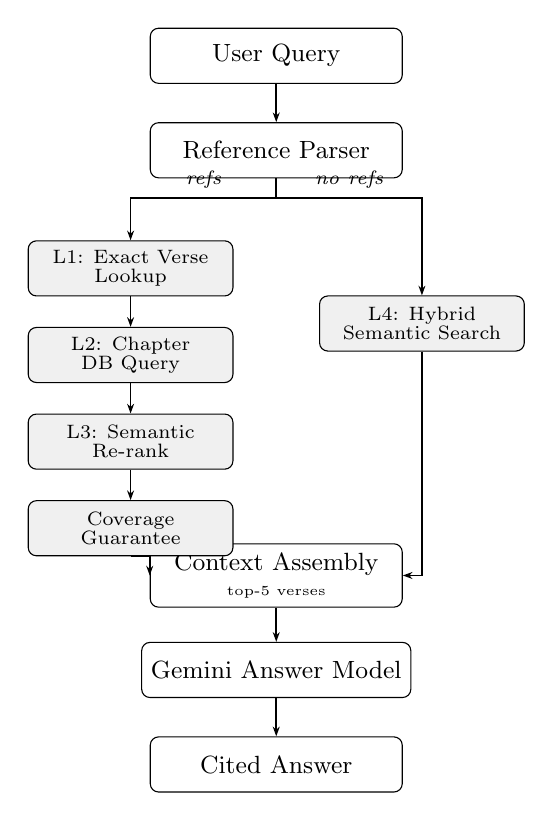
\begin{tikzpicture}[
  spine/.style={draw, rounded corners=3pt, fill=white,
                minimum width=32mm, minimum height=7mm,
                align=center, font=\small},
  layer/.style={draw, rounded corners=3pt, fill=gray!12,
                minimum width=26mm, minimum height=7mm,
                align=center, font=\scriptsize},
  arr/.style={-{Stealth[length=3.5pt,width=2.5pt]}, semithick},
  lbl/.style={font=\scriptsize\itshape}
]
  % Centre spine (x=0)
  \node[spine] at (0, 0)     (q)   {User Query};
  \node[spine] at (0,-1.2)   (p)   {Reference Parser};
  \node[spine] at (0,-6.6)   (ctx) {Context Assembly\\[-2pt]{\tiny top-5 verses}};
  \node[spine] at (0,-7.8)   (mdl) {Gemini Answer Model};
  \node[spine] at (0,-9.0)   (ans) {Cited Answer};

  % Left branch: explicit refs (x=-1.85)
  \node[layer] at (-1.85,-2.7)  (l1) {L1: Exact Verse\\[-1pt]Lookup};
  \node[layer] at (-1.85,-3.8)  (l2) {L2: Chapter\\[-1pt]DB Query};
  \node[layer] at (-1.85,-4.9)  (l3) {L3: Semantic\\[-1pt]Re-rank};
  \node[layer] at (-1.85,-6.0)  (cg) {Coverage\\[-1pt]Guarantee};

  % Right branch: no refs (x=1.85)
  \node[layer] at (1.85,-3.4)   (l4) {L4: Hybrid\\[-1pt]Semantic Search};

  % Spine arrows
  \draw[arr] (q)   -- (p);
  \draw[arr] (ctx) -- (mdl);
  \draw[arr] (mdl) -- (ans);

  % Branch out from parser
  \draw[arr] (p.south) -- ++(0,-0.25)
      -| node[lbl,pos=0.25,above]{refs} (l1.north);
  \draw[arr] (p.south) -- ++(0,-0.25)
      -| node[lbl,pos=0.25,above]{no refs} (l4.north);

  % Left chain
  \draw[arr] (l1) -- (l2);
  \draw[arr] (l2) -- (l3);
  \draw[arr] (l3) -- (cg);

  % Merge into context
  \draw[arr] (cg.south)  -| (ctx.west);
  \draw[arr] (l4.south)  |- (ctx.east);

\end{tikzpicture}
\caption{Aion v3 retrieval pipeline. Queries with explicit scripture references fork left through exact lookup (L1), chapter-aware DB query (L2), in-chapter semantic re-ranking (L3), and a per-chapter coverage guarantee. Queries without references fork right through hybrid semantic search (L4). Both paths merge at context assembly, which selects the top-5 verses for the answer model.}
\label{fig:pipeline}
\end{figure}

\subsection{Reference Parsing}

A two-pass parser identifies explicit scripture references in the query.

\textbf{Pass 1 (verse-level):} Regex matches \texttt{BOOK CHAPTER:VERSE} patterns (e.g., ``John 3:16'', ``Ps.\ 23:1''). An alias map normalizes common abbreviations and alternate spellings to canonical book IDs.

\textbf{Pass 2 (chapter-only):} A separate regex captures patterns like ``Psalm 23'' or ``1 Corinthians 15'' where no verse is specified. A backtrack fix (\texttt{lastIndex = match.index + 1} on alias miss) prevents tokens such as ``Does 1'' from consuming the leading digit of ``1 Corinthians''.

\textbf{Numeric keyword suppression:} Parsed chapter references suppress numeric token extraction in the downstream semantic query. Without this, a query for ``Psalm 23'' generates keyword ``23'', retrieving unrelated numerical content (census records, inventory lists).

\subsection{Layered Retrieval (v3 Direct-Chapter)}

Retrieval proceeds in four layers, ordered by specificity.

\textbf{Layer 1 --- Exact verse lookup.} For verse-level references, the system queries the \texttt{bible\_verses} table directly by (\textit{book\_id}, \textit{chapter}, \textit{verse}). These rows are added to the candidate set without a semantic ranking step.

\textbf{Layer 2 --- Chapter-aware DB query (\texttt{lookupChapterVerses}).} For chapter-only references, all verses in the referenced chapter are fetched directly from \texttt{bible\_verses} by (\textit{book\_id}, \textit{chapter}). This avoids the v2 design flaw of running an unconstrained semantic search then filtering, which could return semantically close verses from other chapters.

\textbf{Layer 3 --- Semantic re-ranking within chapter (\texttt{selectWithinChapters}).} Fetched chapter verses are re-ranked by cosine similarity to the query embedding. An IVFFlat index on the \texttt{embedding} column provides approximate nearest-neighbor search. The top-$k$ results are selected.

\textbf{Per-chapter coverage guarantee.} After semantic re-ranking, the system verifies that at least one verse from each referenced chapter appears in the final candidate set. If not, it appends the chapter's first verse. This ensures multi-hop queries referencing two chapters return at least one verse from each.

\textbf{Layer 4 --- Hybrid semantic fallback.} For queries with no parsed references, the system runs an unconstrained semantic search over all verses using the query embedding. Keywords extracted from the query bias results toward verses with matching lexical content.

\textbf{Context assembly.} The top-5 verses across all layers are assembled into a context block formatted as \texttt{BOOK CHAPTER:VERSE --- \{text\}} on separate lines.

\subsection{Answer Generation}

We pass the assembled verse context and original query to \texttt{gemini-3.1-flash-lite} (Google DeepMind, 2026) with a system prompt that instructs it to: (1) answer using only the provided verses and not recall verses from memory; (2) cite each referenced verse inline using the format \texttt{Book Chapter:Verse}; and (3) acknowledge when the provided verses do not address the question. The prompt contains no explicit instruction to detect false premises or refuse fabrication requests; the 1.000 refusal rate in Table~\ref{tab:main} is an emergent consequence of these three constraints (see Appendix~A).

\subsection{Coarse Retrieval Ablation}

The v1$\rightarrow$v3 progression doubles as a coarse ablation: each version swaps in one retrieval strategy, so the version-over-version deltas indicate the direction of each design change rather than the isolated contribution of a single layer.
v3 matches v2 on the same dataset (R@5\,=\,0.882; Table~\ref{tab:versions}) despite replacing the retrieval architecture.
It fixes aion\_035 (Psalm 23 + John 10 multi-hop) but correctly re-breaks aion\_036, an accidental success in v2 from an unrestricted semantic fallback.

\begin{table}[t]
  \centering
  \small
  \begin{tabular}{llcc}
    \toprule
    \textbf{System} & \textbf{Dataset} & \textbf{R@5} & \textbf{MRR} \\
    \midrule
    v1 hybrid-ref     & v0.1 & 0.676 & 0.552 \\
    v2 chapter-ref    & v0.2 & 0.882 & 0.700 \\
    v3 direct-chapter & v0.2 & 0.882 & 0.714 \\
    v3 direct-chapter & v0.3 & \textbf{0.941} & \textbf{0.773} \\
    \bottomrule
  \end{tabular}
  \caption{Coarse retrieval ablation across system versions. Each version swaps in one retrieval strategy, isolating the direction of each change rather than individual-layer contribution. The v0.3 gain (+0.059 R@5) is attributable to annotation expansion for two questions (aion\_023, aion\_033), not architecture change.}
  \label{tab:versions}
\end{table}

%% ---------------------------------------------------------------
\section{Experiments}
%% ---------------------------------------------------------------

\subsection{Benchmark: Aion-BibleQA gold\_40}

\textbf{Dataset:} \texttt{aion\_bibleqa\_gold\_40\_v0.3.jsonl}, 40 questions across 6 categories (Table~\ref{tab:categories}).
Each question has a \texttt{gold\_verse} (primary expected verse coordinate, e.g., \texttt{JHN.3.16}) and an \texttt{acceptable\_verse\_clusters} list.
R@5\,=\,1 if any retrieved verse matches the gold or any cluster member.
We verified all 40 questions against the live \texttt{bible\_verses} table (BSB translation).

\begin{table}[t]
  \centering
  \small
  \begin{tabular}{@{}p{2.1cm}cp{4.1cm}@{}}
    \toprule
    \textbf{Category} & \textbf{n} & \textbf{Description} \\
    \midrule
    direct        & 10 & Names a specific verse (e.g., ``What does John 3:16 say?'') \\
    interpretive  &  7 & Asks for meaning of a named passage \\
    thematic      & 12 & Theme query without naming a verse \\
    multi\_hop    &  5 & Requires verses from two different chapters \\
    false\_premise &  4 & Contains a factual error about scripture \\
    adversarial   &  2 & Asks the system to fabricate content \\
    \bottomrule
  \end{tabular}
  \caption{Aion-BibleQA category distribution.}
  \label{tab:categories}
\end{table}

\textbf{Annotation note:} Aion-BibleQA is a pilot benchmark created for this study. Questions cover six failure modes identified during v1 system development, not a random sample of user queries. Results should be interpreted in this context.

\subsection{Retrieval Metrics}

\textbf{Recall@5 (R@5):} Binary. Score 1 if any of the top-5 retrieved verse coordinates matches \texttt{gold\_verse} or any cluster member; else 0.

\textbf{MRR (Mean Reciprocal Rank):} $1/r$ where $r$ is the rank of the first matching verse in the ranked list; 0 if no match in top-5.

We compute both metrics per row and report averages per category and overall.

\subsection{Citation-Faithfulness Evaluation}

\textbf{Judge model:} \texttt{gemini-3.1-flash-lite} \citep{google2026gemini31flashlite}.

For each row, the judge receives: (1) the question, (2) the category, (3) expected behavior from the dataset annotation (category-level guidance and refusal expectation, but \emph{not} gold verse coordinates), (4) the retrieved verse block with full verse texts, and (5) the system answer. The judge scored only whether the answer's claims were supported by the cited retrieved verse text; it did not score retrieval relevance against gold annotations.

The judge produces a JSON response with two fields:
\begin{itemize}
  \item \texttt{citation\_support} (0.0--1.0) for direct/interpretive/thematic/multi\_hop rows
  \item \texttt{false\_premise\_refusal} (0 or 1) for false\_premise/adversarial rows
\end{itemize}

\begin{table}[t]
  \centering\small
  \begin{tabular}{@{}cp{6.5cm}@{}}
    \toprule
    \textbf{Score} & \textbf{Meaning} \\
    \midrule
    1.00 & Every claim directly grounded in the cited verse text \\
    0.75 & Mostly grounded; minor over-reach on one citation \\
    0.50 & Some claims go beyond what the verses say \\
    0.25 & Most claims loosely connected to the text \\
    0.00 & Verses decorative; claims unsupported or fabricated \\
    \bottomrule
  \end{tabular}
  \caption{citation\_support scoring rubric used by the LLM judge.}
  \label{tab:rubric}
\end{table}

\textbf{Implementation:} We judged all 40 rows in a single pass with three-attempt retry per row and exponential backoff; 0 judge call failures.

\subsection{Aggregate Metrics}

\begin{itemize}
  \item \textbf{mean\_citation\_support:} Mean cs across non-refusal rows (n\,=\,34)
  \item \textbf{unsupported\_claim\_rate:} Fraction of rows with cs\,<\,0.5
  \item \textbf{decorative\_citation\_rate:} Fraction of rows with cs\,$\leq$\,0.25
  \item \textbf{fp\_refusal\_rate:} Fraction of false\_premise/adversarial rows with false\_premise\_refusal\,=\,1
\end{itemize}

\subsection{Experimental Setup}

Bible translation: BSB (Berean Standard Bible) stored in a Supabase \texttt{bible\_verses} table.
Embedding model: \texttt{text-embedding-3-small} (OpenAI; 1,536 dimensions), stored as \texttt{halfvec(1536)} in pgvector with an IVFFlat index (\texttt{halfvec\_cosine\_ops}).
Answer model: Gemini (same model family as the primary judge; see the Limitations section), deployed as a Supabase Edge Function on Deno Deploy infrastructure.
Judges: \texttt{gemini-3.1-flash-lite} (primary) and OpenAI \texttt{gpt-4.1} (secondary, cross-family robustness check; Section~\ref{sec:multijudge}). Both receive an identical rubric and prompt at temperature 0.1.
Benchmark runner: calls the live Edge Function over HTTPS with SSE streaming from a consumer MacBook.
All benchmark runs are frozen as JSONL artifacts; results are reproducible from those frozen files.

%% ---------------------------------------------------------------
\section{Results}
%% ---------------------------------------------------------------

\subsection{Main Results}

v3 on gold\_40 v0.3 achieves R@5\,=\,0.941, citation\_support\,=\,0.978, and fp\_refusal\,=\,1.000 (Table~\ref{tab:main}), suggesting that once retrieval scope is correct, the system cites retrieved verses faithfully.

\begin{table}[t]
  \centering
  \small
  \begin{tabular}{lc}
    \toprule
    \textbf{Metric} & \textbf{Score} \\
    \midrule
    R@5                            & 0.941 \\
    MRR                            & 0.773 \\
    Mean citation\_support         & 0.978 \\
    Unsupported claim rate (cs\,<\,0.5)   & 0.000 \\
    Decorative citation rate (cs\,$\leq$\,0.25) & 0.000 \\
    False-premise / adversarial refusal & 1.000 (6/6) \\
    \bottomrule
  \end{tabular}
  \caption{v3 system on gold\_40 v0.3: overall metrics.}
  \label{tab:main}
\end{table}

\subsection{Per-Category Breakdown}

\begin{table}[t]
  \centering
  \small
  \begin{tabular}{lccccc}
    \toprule
    \textbf{Category} & \textbf{n} & \textbf{R@5} & \textbf{MRR} & \textbf{cs} & \textbf{fp} \\
    \midrule
    direct        & 10 & 1.000 & 1.000 & 1.000 & --- \\
    interpretive  &  7 & 1.000 & 0.929 & 1.000 & --- \\
    thematic      & 12 & 0.917 & 0.524 & 0.979 & --- \\
    multi\_hop    &  5 & 0.800 & 0.700 & 0.900 & --- \\
    false\_premise &  4 & ---   & ---   & ---   & 1.000 \\
    adversarial   &  2 & ---   & ---   & ---   & 1.000 \\
    \bottomrule
  \end{tabular}
  \caption{Per-category results. cs\,=\,citation\_support; fp\,=\,fp\_refusal. 95\% Wilson CIs for R@5: overall [0.80,\,0.97], multi\_hop [0.38,\,0.96].}
  \label{tab:percat}
\end{table}

\textbf{Direct and interpretive categories.} R@5\,=\,1.00 and citation\_support\,=\,1.00 for all 17 questions (Table~\ref{tab:percat}). The correct verse appears in the top-5 for every question in these categories. MRR\,=\,0.929 for interpretive (vs.\ 1.000 for direct) reflects one question (aion\_006) where the correct verse was retrieved at rank~2; no citation failure resulted.

\textbf{Thematic and multi-hop contain the remaining retrieval failures.} Two questions fail R@5: aion\_027 (thematic, grace semantic drift) and aion\_036 (multi-hop, IVFFlat boundary). Citation faithfulness remains high for both categories (cs\,=\,0.979 and 0.900), showing that the system cites retrieved content correctly even when retrieval returned suboptimal verses.

\textbf{Multi-hop coverage note.} Standard R@5 passes a multi-hop question if \emph{any} required verse is retrieved. Under a stricter per-chapter criterion (success only if every required chapter is represented in the top-5), multi-hop all-chapters recall is also 0.800, but with a different failure: aion\_034 passes standard R@5 (JAS.2.17 retrieved) yet misses the ROM.3 chapter entirely, while aion\_036 has both required chapters present but neither specific gold verse. The two metrics agree on score but expose complementary failure modes.

\textbf{Refusal categories.} All six refusal-category questions scored 1 (4 false-premise, 2 adversarial). No fabricated content appeared in any answer. The adversarial sample (n\,=\,2) is too small for confident generalization; these results are directionally encouraging.

\subsection{Sub-1.0 Rows}

Two rows scored below citation\_support\,=\,1.0.

\textbf{aion\_021} (thematic, cs\,=\,0.75): EPH.6.19 cited for a gratitude context. The verse records Paul requesting prayer for his ministry, not a general statement about thankfulness. A minor over-reach.

\textbf{aion\_035} (multi-hop, cs\,=\,0.50): JHN.10.1 cited instead of JHN.10.11. The per-chapter coverage guarantee appends the first verse of JHN.10 (the parable of the gate) rather than the theologically central verse (``I am the good shepherd''). Notably, R@5\,=\,1 for this question (PSA.23.1 retrieved correctly); the failure is within-chapter verse selection, not retrieval coverage. aion\_035 achieves R@5\,=\,1 yet cs\,=\,0.50, a direct illustration of the retrieval-faithfulness split.

\subsection{Multi-Judge Robustness}
\label{sec:multijudge}

The primary judge (Gemini) shares a model family with the answer model, which risks same-family leniency \citep{zheng2023judging}.
To test whether the headline scores survive a change of judge, we re-scored all 40 rows with a cross-family judge (OpenAI \texttt{gpt-4.1} \citep{openai2025gpt41}) under the identical rubric and prompt (Table~\ref{tab:multijudge}).

\begin{table}[t]
  \centering
  \small
  \begin{tabular}{lcc}
    \toprule
    \textbf{Metric} & \textbf{Gemini} & \textbf{GPT} \\
    \midrule
    Mean citation\_support (n\,=\,34) & 0.978 & 0.941 \\
    Unsupported rate (cs\,<\,0.5)     & 0.000 & 0.000 \\
    Decorative rate (cs\,$\leq$\,0.25) & 0.000 & 0.000 \\
    False-premise refusal             & 1.000 & 1.000 \\
    \bottomrule
  \end{tabular}
  \caption{Two-judge panel on gold\_40 v0.3. The cross-family judge reproduces the unsupported-claim and refusal rates exactly; mean citation\_support differs by 0.037.}
  \label{tab:multijudge}
\end{table}

The two judges agree exactly on 31/40 rows and \emph{within one rubric level on all 40} (every disagreement is a single 0.25 step). Critically, the conclusions that do not depend on a fractional score are judge-invariant: both judges place zero rows below the unsupported threshold and confirm all 6 refusals. The nine disagreements are minor over-reach calls (e.g.\ \texttt{gpt-4.1} rates aion\_021 at 1.00 where Gemini gives 0.75, and the reverse on aion\_027); none crosses a decision boundary. We report this as an automated multi-model robustness check, not as expert human adjudication.

%% ---------------------------------------------------------------
\section{Discussion}
%% ---------------------------------------------------------------

\subsection{The Retrieval-Faithfulness Split}

Retrieval correctness and citation faithfulness are separable.
The two metrics diverge in multi\_hop: R@5\,=\,0.800 while citation\_support\,=\,0.900.
A system can retrieve the wrong verse (R@5\,=\,0) yet cite whatever it retrieved correctly (cs\,=\,1.00): aion\_027 illustrates this.
Conversely, a system can achieve R@5\,=\,1 while citing the wrong verse within a chapter (cs\,=\,0.50): aion\_035 illustrates this.

Both metrics are necessary: high R@5 does not prevent unsupported-citation failures, and high citation\_support does not confirm that retrieved content was relevant. We use ``citation misuse'' to mean citing verses that are decorative or do not support the stated claim; aion\_035 is not this kind of failure (JHN.10.1 was retrieved and cited faithfully; the per-chapter guarantee returned the wrong verse within the correct chapter).

\subsection{Failure Taxonomy}

All remaining failures fall into one of three classes (Table~\ref{tab:failures}).

\begin{table}[t]
  \centering
  \small
  \begin{tabular}{@{}p{1.8cm}p{2.8cm}p{2.0cm}@{}}
    \toprule
    \textbf{Class} & \textbf{Example} & \textbf{Fix} \\
    \midrule
    Semantic drift & aion\_027: ``grace'' $\rightarrow$ salutation formulas & Query expansion + salutation penalty (v3.1) \\
    IVFFlat boundary & aion\_036: PHP.4.6 inconsistently absent & Per-chapter vector RPC (v4) \\
    Per-chapter wrong verse & aion\_035: JHN.10.1 vs JHN.10.11 & Per-chapter vector RPC (v4) \\
    \bottomrule
  \end{tabular}
  \caption{Remaining failure taxonomy. None is an unsupported-citation or decorative-citation failure; the system does not fabricate verse support. aion\_035 scores cs\,=\,0.50 because the per-chapter guarantee returned the wrong verse within the correct chapter, not because the model cited a verse it did not retrieve.}
  \label{tab:failures}
\end{table}

In every case where retrieval returned relevant content, the answer model cited it correctly.
Fixing retrieval scope addresses both remaining failure classes.

\subsection{The aion\_027 Grace Drift}

``Grace'' in Pauline letters has two semantic neighborhoods: salvific grace (EPH.2.8--9: ``For by grace you have been saved through faith'') and epistolary grace (greeting formulas of the form ``Grace and peace to you\ldots'').
The epistolary cluster dominates the embedding space: these short, formulaic verses have embeddings closer to the unqualified query ``grace'' than the longer salvific passage.

Two candidate fixes: (1) query expansion, prepending ``saved by'' or ``salvation'' to thematic grace queries at retrieval time; (2) salutation suppression, a post-retrieval filter penalizing verses matching the pattern ``Grace and peace to you from X''.
The second is more targeted; the first generalizes more broadly to other semantic drift cases.

\subsection{v4 Architecture Roadmap}

aion\_035 and aion\_036 share a root cause: the per-chapter guarantee and IVFFlat search operate at chapter granularity, not verse-within-chapter granularity.

The v4 fix is a \texttt{search\_verses\_in\_chapter} Supabase RPC running constrained vector search within a single chapter, parameterized by query embedding, book ID, chapter number, and return count $k$.
For JHN.10, the intended effect is that a query embedding for ``God as shepherd'' would rank JHN.10.11 above JHN.10.1; this has not been experimentally confirmed.
The per-chapter guarantee would then return the semantically best verse within the chapter rather than the chapter's first verse.
This is a well-defined engineering task with a clear specification derived from the failure analysis.

%% ---------------------------------------------------------------
\section{Conclusion}
%% ---------------------------------------------------------------

We introduced Aion-BibleQA, a 40-question benchmark for citation-faithfulness and false-premise robustness in verse-grounded Bible RAG.
Our v3 retrieval system, combining exact verse lookup, direct chapter-aware database queries, per-chapter coverage guarantees, and hybrid semantic re-ranking, achieves R@5\,=\,0.941 on gold\_40 v0.3.
A Gemini LLM-as-judge evaluation shows mean citation\_support\,=\,0.978, zero unsupported citations, and a 1.000 false-premise refusal rate.

Retrieval and citation faithfulness are distinct failure modes.
In this pilot, citation failures disappear when the retrieved verse set contains the required evidence.
The remaining errors (semantic drift in thematic queries, IVFFlat boundary effects in multi-hop retrieval, and within-chapter verse selection) are retrieval scope problems.

Future priorities:
\begin{itemize}
  \item Expert (theological) human annotation, beyond the automated cross-family judge agreement already reported.
  \item Expansion to 200+ questions sampled from real users.
  \item Thematic query expansion for grace-like semantic drift (v3.1).
  \item Per-chapter vector search RPC for within-chapter verse selection (v4).
\end{itemize}

We release Aion-BibleQA, the retrieval system, the judge harness, and all benchmark artifacts alongside this paper at \url{https://github.com/Raoof128/Aion} (code) and \citep{aion2026benchmark} (frozen dataset, Zenodo DOI: \href{https://doi.org/10.5281/zenodo.20522874}{10.5281/zenodo.20522874}).

%% ---------------------------------------------------------------
\section*{Limitations}
%% ---------------------------------------------------------------

\textbf{Automated judging, no expert human validation.} Citation-faithfulness scores come from LLM judges, and the primary judge (Gemini) shares a model family with the answer model, which risks same-family leniency \citep{zheng2023judging}. We mitigate this with a cross-family judge (\texttt{gpt-4.1}) on all 40 rows: the two judges agree within one rubric level on every row and report identical unsupported-claim and refusal rates (Section~\ref{sec:multijudge}), so the headline conclusions are robust to the choice of judge. We do not, however, claim expert theological validation: we evaluate only whether generated claims are supported by the cited verse text, under a reproducible multi-model protocol. Expert human annotation, and a larger automated panel (a third judge harness is included but unrun for lack of an API key), remain future work.

\textbf{Pilot benchmark size.} gold\_40 v0.3 contains 40 questions. Statistical uncertainty is high: R@5 is averaged over the 34 non-refusal rows, so one question shifts it by roughly 3\% (1 of 34). Results in the multi\_hop category (n\,=\,5) and adversarial category (n\,=\,2) are especially noisy. A 95\% CI on multi\_hop R@5\,=\,0.800 with n\,=\,5 spans roughly $\pm$0.30.

\textbf{Constructed benchmark, not user-sampled.} Questions target known failure modes from v1 development, not the distribution of queries real users ask. The benchmark was created by the same team that built the system under evaluation; scores may overstate performance relative to an independently assembled evaluation set. Real-world R@5 may differ.

\textbf{Single translation (BSB).} All verses come from the Berean Standard Bible. Results may not generalize to systems using KJV, NIV, ESV, or other translations, where verse wording differs and embeddings shift.

\textbf{IVFFlat non-determinism.} Across three repeated runs on gold\_40 v0.2, three questions showed R@5 variance (aion\_006, aion\_007, aion\_036). Run-to-run R@5 ranged from 0.853 to 0.882 on the same question set. Benchmark runs in this paper were each performed once and frozen as canonical JSONL artifacts; results are reproducible from those frozen files.

\textbf{Coarse, not controlled, ablation.} The v1$\to$v2$\to$v3 progression (Table~\ref{tab:versions}) acts as a coarse ablation showing the direction of each design change, but each version alters more than one component at once, so the isolated contribution of an individual retrieval layer is not quantified.

%% ---------------------------------------------------------------
\section*{Acknowledgments}
%% ---------------------------------------------------------------

We thank the Berean Bible translators for dedicating the BSB to the public domain with all uses freely permitted, which made this corpus-based study possible.

%% ---------------------------------------------------------------
\section*{Ethics Statement}
%% ---------------------------------------------------------------

This study uses the Berean Standard Bible (BSB), whose texts are dedicated to the public domain with all uses freely permitted.
No personal data were collected; Aion-BibleQA contains no human subject information.
The judge and answer models are commercial APIs; no model weights were modified or redistributed.
The benchmark targets a low-risk religious reference task; nonetheless, retrieval failures that misattribute scripture could mislead users about biblical content, and results should not be interpreted as endorsing any theological position.

%% ---------------------------------------------------------------
\bibliography{paper}
%% ---------------------------------------------------------------

\appendix

%% ---------------------------------------------------------------
\section{Answer Generation System Prompt}
\label{app:prompt}
%% ---------------------------------------------------------------

The following prompt is used verbatim by \texttt{buildPrompt()} in
\texttt{supabase/functions/chat/index.ts}.
\texttt{\{versesBlock\}} is populated at runtime with the top-5 retrieved
verses formatted as \texttt{BOOK CH:VS --- "text"} on separate lines;
\texttt{\{userMessage\}} is the verbatim user query.

\begin{quote}
\small
\texttt{You are Aion, a wise and warm Bible companion. You help people explore
Scripture with clarity and warmth.}

\texttt{RULES:}\\
\texttt{- Answer using ONLY the provided verses below. Do not invent or recall}\\
\texttt{\ \ verses from memory.}\\
\texttt{- Cite each verse you reference using the format: Book Chapter:Verse.}\\
\texttt{- If the provided verses don't answer the question, say so honestly and}\\
\texttt{\ \ suggest what the user might search for instead.}\\
\texttt{- Keep your response concise and conversational (2-4 short paragraphs max).}

\texttt{[Retrieved Verses]}\\
\texttt{\{versesBlock\}}

\texttt{[User Question]}\\
\texttt{\{userMessage\}}
\end{quote}

\textbf{Design note.}
The prompt contains no explicit false-premise detection or fabrication-refusal instruction.
The refusal behavior follows from the grounding-only constraints: Rule~1 prohibits recalled knowledge; when the retrieved verse block contains no relevant content (as occurs for non-existent passages or adversarial queries), Rule~3 produces a natural refusal. Robustness to false premises is therefore a consequence of the retrieval constraints rather than an explicitly programmed detection rule.

\end{document}
